%
% vergleich.tex
%
% (c) 2021 Prof Dr Andreas Müller, OST Ostschweizer Fachhochschule
%
\documentclass[tikz]{standalone}
\usepackage{times}
\usepackage{amsmath}
\usepackage{txfonts}
\usepackage[utf8]{inputenc}
\usepackage{graphics}
\usetikzlibrary{arrows,intersections,math}
\usepackage{ifthen}
\begin{document}

\newboolean{showgrid}
\setboolean{showgrid}{false}
\def\breite{5}
\def\hoehe{5}

\begin{tikzpicture}[>=latex,thick]

% Povray Bild
\node at (0,0) {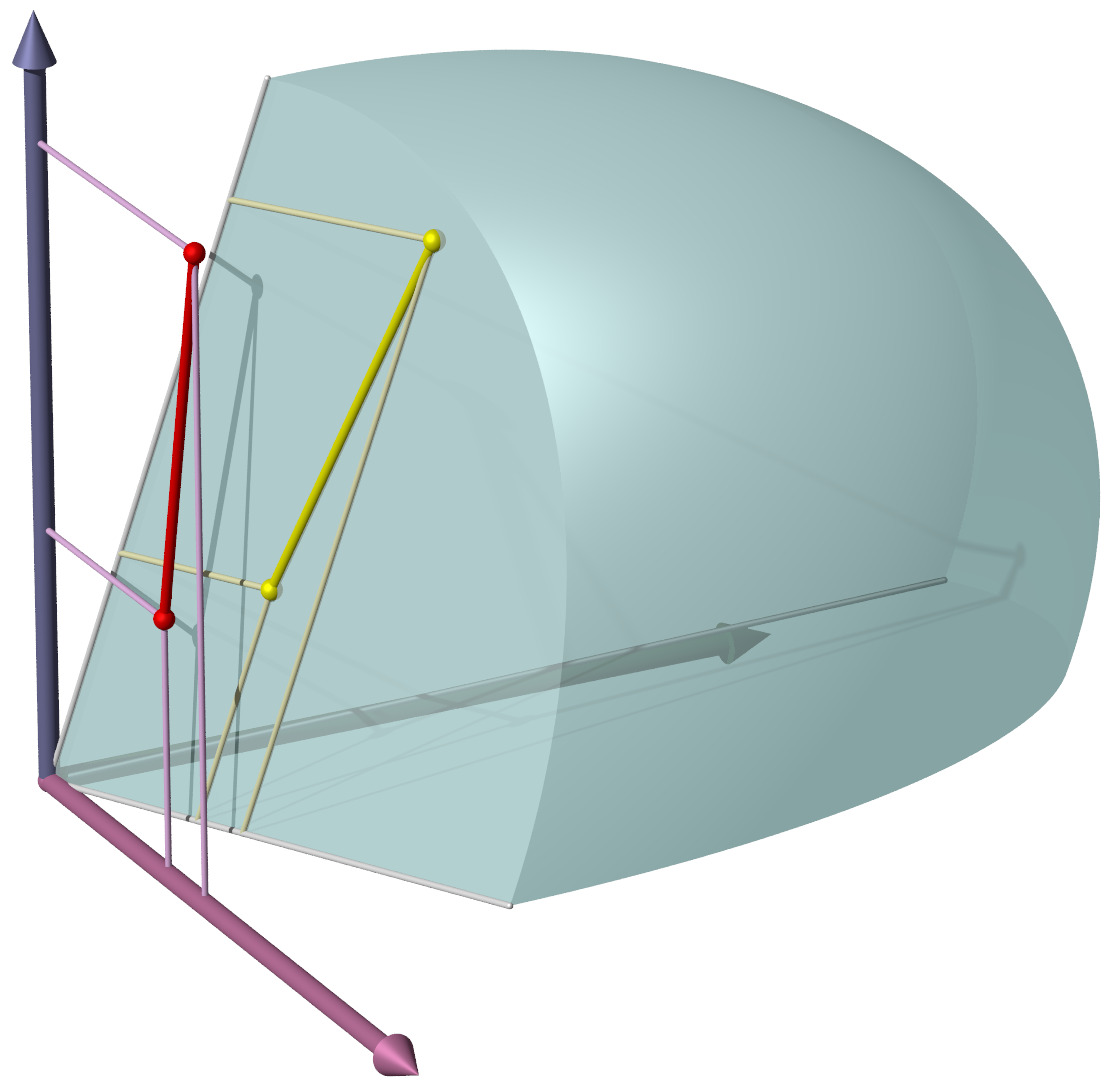
\includegraphics[width=10cm]{vergleich.jpg}};

\node at (-1.3,-4.8) [right] {$x_1$};
\node[opacity=0.5] at (1.9,-0.9) [right] {$x_2$};
\node at (-4.6,4.7) [right] {$x_3$};

\node at (-3.2,2.6) [above] {$u$};
\node at (-3.5,-0.7) [below left] {$v$};
\node at (-1,2.8) [above] {$Au$};
\node at (-2.6,-0.5) [below] {$Av$};

% Gitter
\ifthenelse{\boolean{showgrid}}{
\draw[step=0.1,line width=0.1pt] (-\breite,-\hoehe) grid (\breite, \hoehe);
\draw[step=0.5,line width=0.4pt] (-\breite,-\hoehe) grid (\breite, \hoehe);
\draw                            (-\breite,-\hoehe) grid (\breite, \hoehe);
\fill (0,0) circle[radius=0.05];
}{}

\end{tikzpicture}

\end{document}

